\documentclass[11pt]{article}
\usepackage[margin=1in]{geometry}
\usepackage{amsmath,amssymb,amsthm,mathtools}
\usepackage{booktabs,enumitem,graphicx,xcolor}
\usepackage{xurl}
\usepackage[section]{placeins}
\usepackage[colorlinks=true,linkcolor=blue!50!black,citecolor=green!35!black,urlcolor=blue!50!black]{hyperref}
\usepackage[nameinlink]{cleveref}
\newtheorem{theorem}{Theorem}\newtheorem{proposition}[theorem]{Proposition}\newtheorem{lemma}[theorem]{Lemma}\newtheorem{corollary}[theorem]{Corollary}
\theoremstyle{definition}\newtheorem{definition}[theorem]{Definition}\newtheorem{remark}[theorem]{Remark}\newtheorem{example}[theorem]{Example}
\newcommand{\R}{\mathbb R}
\setlength{\emergencystretch}{3em}
\title{Two Latent Types on Arbitrary Covers\\[2pt]\large Part I: pair graphs, sign sheets and hiding polytopes\\ \normalsize (working draft: Phases I--III; three types)}
\author{Vinay K Awasthi\\ Johns Hopkins University\\ \texttt{vawasth1@jh.edu}}
\date{October 2026}
\begin{document}
\maketitle

\begin{abstract}
The lab for latent actors \cite{Lab} proved its two-type results mostly on the complete pair cover of three or four variables. This
companion asks the same questions for an arbitrary graph $G$ of observed pairs on $m$ binary variables. When do the pair tables admit a
two-type explanation? Which freedoms remain? What does the set of explanations look like? This draft answers them at the pair layer, then for higher windows and for three types.
\begin{itemize}
\item \emph{Existence} (\cref{thm:factor}). A factorisation $c_{ij}=v_iv_j$ exists iff three conditions hold. No zero moment may join
  two variables that carry non-zero moments. On each component of the non-zero graph $G^*$, the sign cocycle must be a $\mathbb Z/2$
  coboundary, and $\log|c|$ must lie in the image of the unsigned incidence matrix. The last two are the lab's $H^1_+=H^1(\Gamma;\mathbb
  Z/2)\oplus\operatorname{coker}B$, extended to any graph.
\item \emph{Freedom.} $\operatorname{rank}B_G=m-b(G)$, with $b(G)$ the number of bipartite components (isolated vertices included).
  Odd cycles pin the magnitudes. Each bipartite component keeps a scale $\lambda^{\pm1}$. Each component keeps its own sign, so the
  labels can be swapped on one component alone, invisibly to the pairs.
\item \emph{Hiding polytopes} (\cref{thm:hiding}). The two-type explanations fall into sign sheets. In the coordinates $y=\log t$ (the
  weight) and $x_k=\log\lambda_k$, each sheet is a convex polytope whose facets all have slope $\pm1$, two per variable: the positivity
  walls $a_{1i},a_{2i}\in\{0,1\}$. For a connected bipartite graph the sheet is a rectangle in $(\log\lambda t,\log\lambda/t)$. The
  generic dimension is $b(G)+1$. The label swap identifies sheets in pairs. Positivity can empty a sheet.
\item \emph{Strata.} A coincidence $v_i=0$ deletes vertex $i$ from $G^*$. On the triangle it leaves a single edge, so the lab's hiding
  segment becomes a two-dimensional region.
\item \emph{Relations and syzygies} (Phase III, Stage 1, \cref{thm:syz}). With triple windows the moment map is monomial, so the
  relations among observed moments form the toric ideal of the extended incidence matrix. Each triple either is absorbed or adds one
  test. Relations are disconnected fibres and syzygies are hollow loops (Hochster's formula). The syzygies are exactly the dependencies
  among the tests, so a test of all relations has $\operatorname{codim}$ degrees of freedom. On the bowtie the ideal is Hilbert--Burch:
  three witnesses of one latent ratio. A coincidence on a shared variable disables the tests that pass through it.
\item \emph{Higher windows and three types} (\cref{thm:higher,prop:collinear,prop:three}). The polynomials $s_k(r)$ are the moments
  of a standardised two-point latent, so higher windows obey Fibonacci gluing relations whose two-triple case is a Hankel determinant.
  For collinear $k$ types the hiding set is a moment space. Two types are its lower boundary, so the lab's quadruple residual becomes a
  one-sided test for more types. Under pair-only disclosure three-variable events have the same range for any number of collinear
  types. For three types on five variables, a single four-window is defective but two overlapping ones identify the law: $S_3$ descent.
\item \emph{Real signs} (\cref{thm:signs}). The sign symmetries are the kernel of a parity matrix over $\mathbb F_2$. The lab's sign group
  splits into classes the relations see (their sign shadows) and odd-cycle classes no relation can see (the $2$-torsion of the Smith
  form). Syzygies evaluated at the torus identity are the dependencies among the sign tests. A sheet lost on the latent side is a sign
  test gained on the data side.
\item \emph{Strata} (\cref{thm:strata}). Ranks drop by an explicit rule: faces avoiding the coincident set give the latent rank, and the
  number of factors through a variable decides which tests survive. On pair graphs a coincidence costs one degree of freedom per extra
  non-bipartite lobe; a cut vertex alone costs nothing. Equal weights un-align labels that travelled through $r$.
\end{itemize}
Forty-one checks (CV1--CV9, SZ1--SZ8, HW1--HW8, SG1--SG8, CS1--CS8) verify every statement: on a zoo of eleven graphs, by sampling each polytope and rebuilding the
law; on eight covers, by recomputing every Betti number from Hochster's formula; and on the higher windows, by recomputing every
Betti table in a second computer-algebra system. The identifiability notions and walls (Phases IV--V), and the general three-type theory on arbitrary covers follow.
\end{abstract}

\section{Setting}\label{sec:setting}
Variables are $0,\dots,m-1$. A two-type law has weight $w$ and success probabilities $a_1,a_2\in[0,1]^m$, with
\[
\mu=wa_1+(1-w)a_2,\qquad v=\sqrt{w(1-w)}\,(a_1-a_2),\qquad c_{ij}=\operatorname{Cov}(X_i,X_j)=v_iv_j .
\]
Following the lab, write $t=\sqrt{(1-w)/w}$, so that $w=1/(1+t^2)$, $a_1=\mu+vt$ and $a_2=\mu-v/t$. The label swap is
$(v,t)\mapsto(-v,1/t)$. Observed are the single tables, which give $\mu$, and the pair tables on the edges $E$ of a graph $G=(V,E)$,
which give $c_e$. On $K_3$ the explanations form the lab's hiding segment \cite[Theorem A]{Lab}. Here $G$ is arbitrary: possibly
disconnected, bipartite or not, with zero moments allowed.

Write $B_G$ for the unsigned incidence matrix ($E\times V$, with a $1$ where the vertex lies on the edge), and $b(G)$ for the number of
bipartite components, an isolated vertex counting as one.

\begin{lemma}[rank]\label{lem:rank}
$\operatorname{rank}B_G=|V|-b(G)$. The kernel is spanned, for each bipartite component with sides $L,R$, by the vector that is $+1$ on
$L$, $-1$ on $R$ and $0$ elsewhere. An isolated vertex contributes its own coordinate.
\end{lemma}

\begin{proof}
A vector $x$ lies in the kernel iff $x_i=-x_j$ on every edge. Along a path $x$ alternates in sign. On a component with an odd cycle this
forces $x=0$; on a bipartite component it forces $\pm a$ on the two sides. Check CV1 verifies the formula on $300$ random graphs.
\end{proof}

\section{Phase I: the factorisation on any pair graph}\label{sec:factor}
For data $c\in\R^E$, let $N$ be the set of vertices on some edge with $c_e\ne0$, and $G^*=(N,\{e:c_e\ne0\})$ the non-zero graph. Let $Z$ be
the vertices outside $N$ joined to $N$ by a zero edge, and $F=V\setminus(N\cup Z)$ the \emph{free} vertices.

\begin{theorem}[factorisation]\label{thm:factor}
A real $v$ with $v_iv_j=c_{ij}$ for every edge exists iff the following hold.
\begin{enumerate}
\item[(i)] \emph{Zero strata.} No edge with $c_e=0$ joins two vertices of $N$.
\item[(ii)] \emph{Sign class.} On each component $H$ of $G^*$, the cochain $\operatorname{sgn}c|_H\in C^1(H;\mathbb Z/2)$ is a coboundary.
  Equivalently, the product of the $c_e$ around every cycle is positive. This is $b_1(H)$ conditions.
\item[(iii)] \emph{Modulus class.} On each component $H$, $\log|c|_H\in\operatorname{im}B_H$, that is, it is orthogonal to
  $\ker B_H^\top$. This is $|E_H|-|V_H|+\beta_H$ equations, with $\beta_H=1$ if $H$ is bipartite and $0$ otherwise.
\end{enumerate}
When they hold, the set of factorisations is
\[
\mathcal F_G(c)=\prod_{H}\mathcal F_H\times\{0\}^Z\times\mathcal S_F ,
\]
where:
\begin{itemize}
\item $\mathcal F_H=\{\pm v_H\}$ if $H$ is not bipartite;
\item $\mathcal F_H=\{\sigma\lambda^{\varepsilon}v_H:\sigma=\pm1,\ \lambda>0\}$ if $H$ is bipartite, where $\varepsilon_i=\pm1$ marks
  the side of $i$;
\item $\mathcal S_F$ is the set of $v\in\R^F$ with $v_iv_j=0$ on the zero edges inside $F$: the union of the coordinate subspaces of the
  independent sets of that graph.
\end{itemize}
In particular the components' signs are independent, and the tangent dimension of $\prod_H\mathcal F_H$ is the number of bipartite
components of $G^*$.
\end{theorem}

\begin{proof}
(i) If $v_iv_j=0$, one of $v_i,v_j$ is zero, but a vertex of $N$ has a non-zero product with a neighbour, so it is not zero. This also
forces $v=0$ on $Z$. On $G^*$, write $v_i=\sigma_i e^{x_i}$. Then $v_iv_j=c_{ij}$ splits into $\sigma_i\sigma_j=\operatorname{sgn}c_{ij}$,
the coboundary condition (ii) over $\mathbb Z/2$, and $x_i+x_j=\log|c_{ij}|$, the condition $B_Hx=\log|c|$ of (iii). The two systems
are independent, and \cref{lem:rank} gives their solution sets: $\sigma$ up to a global sign per component, and $x$ up to the kernel of
$B_H$. The dimension of (ii) is the cycle rank $b_1(H)$; the codimension of $\operatorname{im}B_H$ is $|E_H|-\operatorname{rank}B_H$.
On $F$ only the zero edges constrain. Check CV2 compares the criterion with a direct non-linear solve on $66$ cases (each graph in the
zoo, with true, sign-corrupted and modulus-corrupted data): it agrees in all of them. Check CV3 confirms the dimension count on the zoo.
\end{proof}

\begin{remark}[relation to the lab's descent tower]
On a connected pair graph, (ii) and (iii) together are Theorem M of the lab, $H^1_+=H^1(\Gamma;\mathbb Z/2)\oplus\operatorname{coker}B$
\cite[Theorem M]{Lab}. On $K_4$, $\operatorname{coker}B$ is two-dimensional and spanned by the log tetrads. Three cases are new here:
disconnected graphs, where the sign group becomes $(\mathbb Z/2)^{\#\text{components}}$; bipartite graphs, which have an extra kernel
direction; and zero strata. On the 4-cycle, (iii) is the single equation $|c_{01}c_{23}|=|c_{12}c_{03}|$, an even-cycle tetrad. On odd
cycles (iii) is empty.
\end{remark}

\begin{remark}[labels on one component]
If $G^*$ has several components, flipping the sign of $v$ on one component swaps the two types' labels there and only there. This is a
two-type law with the same pairs but a different joint law. It is not a symmetry of the model; the windows of Part II detect it exactly
when they join components with an odd count on each side (\cref{sec:next}).
\end{remark}

\section{Phase II: the hiding set}\label{sec:hiding}
Fix the component signs $\sigma\in\{\pm1\}^{\#\text{comp}(G^*)}$, a sheet. Write $y=\log t$ and $x_k=\log\lambda_k$ for the bipartite
components, and choose a base factorisation $v_H$ on each component. A vertex $i\in N$ then has $v_i=s_ia_ie^{z_i}$, with $a_i=|v_{H,i}|$,
sign $s_i$ and $z_i=\varepsilon_ix_k$ ($z_i=0$ on rigid components).

\begin{theorem}[hiding polytopes]\label{thm:hiding}
The two-type explanations of $(\mu,c)$ on $G$ are the points $(\sigma,y,x)$ with $(y,x)\in\Pi_\sigma$, together with a value $v_i$ for
each free vertex in the interval
\[
J_i(t)=\bigl[\max(-\mu_i/t,\,-(1-\mu_i)t),\ \min((1-\mu_i)/t,\,\mu_i t)\bigr]\ni0 ,
\]
subject to $\mathcal S_F$. Here $\Pi_\sigma$ is cut out by two inequalities per vertex $i\in N$:
\[
\begin{array}{lll}
s_i>0: & z_i+y\le\log\frac{1-\mu_i}{a_i}\ (a_{1i}\le1), & z_i-y\le\log\frac{\mu_i}{a_i}\ (a_{2i}\ge0),\\[3pt]
s_i<0: & z_i+y\le\log\frac{\mu_i}{a_i}\ (a_{1i}\ge0), & z_i-y\le\log\frac{1-\mu_i}{a_i}\ (a_{2i}\le1).
\end{array}
\]
\begin{enumerate}
\item[(1)] Each $\Pi_\sigma$ is a convex polytope, and every facet normal has the form $(\pm1,\pm e_k)$ or $(\pm1,0)$: slope $\pm1$ in
  each plane $(y,x_k)$.
\item[(2)] If $G$ is connected and bipartite, $\Pi$ is the rectangle
\[
-\min_{R}\beta_i\le u\le\min_L\alpha_i,\qquad -\min_R\alpha_i\le w\le\min_L\beta_i,
\]
  where $u=x+y=\log\lambda t$, $w=x-y=\log\lambda/t$, and $\alpha_i,\beta_i$ are the right-hand sides of the first and second rows.
  Type~1 on $L$ deviates by $e^{u}$ and type~2 on $R$ by $e^{-u}$ (times the base); type~2 on $L$ by $e^{w}$ and type~1 on $R$ by
  $e^{-w}$. The two products move independently.
\item[(3)] If every $c_e\ne0$ and the truth has $a_{1i},a_{2i}\in(0,1)$ for all $i$, the truth lies in the interior of its sheet. The
  hiding set then has dimension $b(G)+1$: one for $t$, one for each bipartite scale, one for each isolated vertex.
\item[(4)] The label swap maps $\Pi_\sigma$ to $\Pi_{-\sigma}$ by $y\mapsto-y$, so there are $2^{c^*-1}$ distinct sheets, $c^*$ being
  the number of components of $G^*$. Positivity can empty a sheet.
\item[(5)] On $K_3$ the single sheet is $y\in[\log t_-,\log t_+]$, the lab's hiding segment.
\end{enumerate}
\end{theorem}

\begin{proof}
Given $v\in\mathcal F_G(c)$ and $t>0$, the law $(w,a_1,a_2)$ reproduces $\mu$ and all $c_e$ by construction. It is a law iff
$a_1,a_2\in[0,1]^m$. For $v_i=s_ia_ie^{z_i}$ with $s_i>0$, the active bounds are $a_{1i}=\mu_i+a_ie^{z_i}t\le1$ and
$a_{2i}=\mu_i-a_ie^{z_i}/t\ge0$; taking logs gives the display, and $s_i<0$ is symmetric. Conversely, every explanation has $v\in\mathcal
F_G(c)$ and some $t$, by \cref{thm:factor}. For a free vertex the bounds are linear in $v_i$ and contain $0$.
(1) The constraints are linear in $(y,x)$.
(2) On $L$, $z=x$ and the rows read $u\le\alpha_i$, $w\le\beta_i$. On $R$, $z=-x$ and they read $-w\le\alpha_i$, $-u\le\beta_i$.
(3) Strict inequalities at the truth give an open neighbourhood. The coordinates are $y$, one $x_k$ per bipartite component of $G^*$
($=G$ minus its isolated vertices), and one $v_i$ per isolated vertex. These number $b(G)+1$.
(4) $v\mapsto-v$ flips every $s_i$, and $t\mapsto1/t$ exchanges the two rows of each vertex.
(5) $K_3$ has no scale, and the rows reduce to the lab's $t_-=\max(\ldots)$, $t_+=\min(\ldots)$ \cite[Theorem A]{Lab}.
Check CV5 samples every sheet of every zoo graph by hit-and-run. Each point rebuilds a law with exactly the observed singles and pairs
and $a\in[0,1]^m$, and stepping $10^{-3}$ beyond any facet takes the named $a_{1i}$ or $a_{2i}$ out of $[0,1]$. Checks CV6--CV9 verify
(2)--(5).
\end{proof}

\begin{figure}[t]\centering
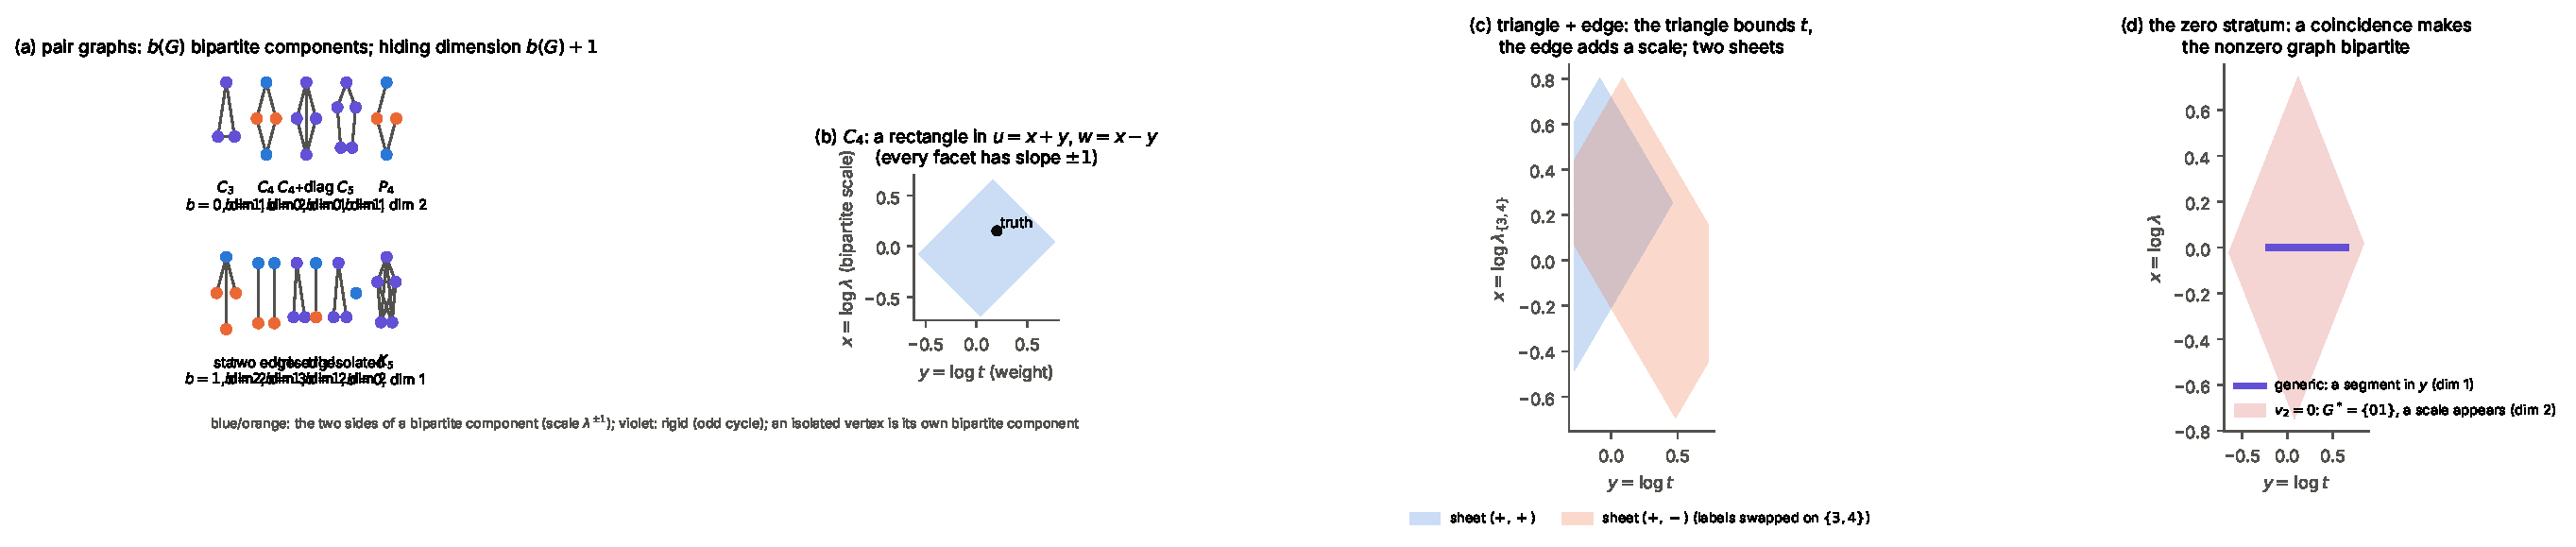
\includegraphics[width=\textwidth]{fig_zoo.pdf}
\caption{Phases I--II. (a) The zoo, with the two sides of each bipartite component coloured. The hiding dimension is $b(G)+1$
throughout (CV7). (b) $C_4$: the sheet in $(y,x)=(\log t,\log\lambda)$ is a rectangle turned $45^\circ$, a rectangle in
$(\log\lambda t,\log\lambda/t)$ (\cref{ex:c4}). (c) Triangle plus a disjoint edge: the triangle bounds $t$ and the edge adds a scale. The
two sheets differ by swapping the labels on $\{3,4\}$ only. (d) The triangle generically has a one-dimensional sheet (the lab's segment).
At the coincidence $v_2=0$ the non-zero graph is the single edge $01$, which is bipartite, and the sheet becomes two-dimensional.}
\label{fig:zoo}
\end{figure}

\section{Worked examples}\label{sec:worked}
\begin{example}[$C_4$, every step]\label{ex:c4}
Take $w=0.4$, $a_1=(0.8,0.3,0.7,0.25)$ and $a_2=(0.2,0.7,0.15,0.7)$, observed on the 4-cycle $01,12,23,03$.
\begin{enumerate}
\item \emph{Data.} $\mu=(0.44,0.54,0.37,0.52)$ and $v=(0.2939,-0.1960,0.2694,-0.2205)$, so
  $c_{01}=-0.0576$, $c_{12}=-0.0528$, $c_{23}=-0.0594$ and $c_{03}=-0.0648$.
\item \emph{Existence.} The sign product around the cycle is $(-)^4>0$, so (ii) holds. The single modulus equation is
  $c_{01}c_{23}/(c_{12}c_{03})=1.0000$, so (iii) holds.
\item \emph{Factorisation.} The sides are $L=\{0,2\}$ and $R=\{1,3\}$. The minimum-norm base solution is
  $v_H=(0.2526,-0.2280,0.2316,-0.2565)$, and the truth is $\lambda=1.1636$ times it on $L$ and $\lambda^{-1}$ times it on $R$.
\item \emph{The rectangle.} The eight rows give
\[
u=\log\lambda t\in[-0.627,\,0.796],\qquad w=\log\lambda/t\in[-0.707,\,0.469].
\]
  The binding walls are $a_{1,0}\le1$ and $a_{2,3}\le1$ for $u$, and $a_{2,2}\ge0$ and $a_{1,3}\ge0$ for $w$.
\item \emph{The truth.} $t=\sqrt{0.6/0.4}=1.2247$, so $y=0.2027$, $x=\log1.1636=0.1515$, $u=0.354$ and $w=-0.051$: inside, as
  \cref{fig:zoo}(b) shows.
\end{enumerate}
So the 4-cycle leaves two dimensions free. A triple window on $\{0,1,2\}$ meets $L$ twice and $R$ once, so it constrains
$\log|v_{012}|=x+\text{const}$, and through $s_3(r)$ also $y$. It removes one dimension; a second triple $\{1,2,3\}$ removes the
other (\cref{sec:next}).
\end{example}

\begin{example}[two disjoint edges: a sheet killed by positivity]\label{ex:kill}
Take edges $01$ and $23$, with $w=0.9$, $a_1=(0.05,0.02,0.15,0.05)$ and $a_2=(0.55,0.45,0.75,0.90)$. There are two components, each
bipartite, so there are $2^{2-1}=2$ sheets, in three dimensions $(y,x_1,x_2)$. The true sheet has dimension $3$. The other sheet, with the
labels swapped on $\{2,3\}$, is empty. Swapping labels on one block would require that block's weight to be $0.1$, so it needs
$t\mapsto1/t$ there. But $t$ is shared, and the block's scale cannot compensate within the walls (CV9). Under less extreme weights both
sheets are realised; in \cref{fig:zoo}(c) both sheets of the triangle-plus-edge are non-empty.
\end{example}

\begin{example}[the zero stratum on the triangle]\label{ex:zero}
With $a_1=(0.8,0.3,0.6)$, $a_2=(0.2,0.7,0.6)$ and $w=0.4$, the variable $2$ is a coincidence: $v_2=0$, so $c_{02}=c_{12}=0$. Then
$N=\{0,1\}$, $Z=\{2\}$ and $G^*=\{01\}$, which is bipartite. The lab's segment becomes the two-dimensional region of
\cref{fig:zoo}(d). The weight is no longer tied to a one-parameter curve, because nothing links the scale of $v_0$ to that of $v_1$
except their product. If instead $c_{01}=0$ while $c_{02},c_{12}\ne0$, condition (i) fails and no factorisation exists (CV4).
\end{example}

\section{Phase III, Stage 1: relations and their syzygies}\label{sec:syz}
Phase III is done in stages. Stage 1, this section, treats covers by pairs and triples, where the moment map is monomial. Stage 2 will
add windows of size four and more, where $s_k(r)$ is no longer a monomial. Stage 3 handles real signs and parities. Stage 4 handles strata.

\paragraph{Algebra, reals and positivity.} Before the relations, here is how they relate to the hiding polytopes. Write
$\varphi:(v,r)\mapsto(m_F)_F$ for the moment map from latent to observed coordinates.

\begin{lemma}[algebra, reals, positivity]\label{lem:bridge}
\begin{enumerate}
\item[(1)] \emph{Algebra (data side).} The relations of the cover generate the ideal $I_A$ of the Zariski closure of the image of $\varphi$.
  Data off $V(I_A)$ have no explanation, even over $\mathbb C$.
\item[(2)] \emph{Algebra (latent side).} Over data in the image with all moments non-zero, the fibre $\varphi^{-1}(c)$ is a coset of the
  torus $K=\{z:z^{a_j}=1\text{ for all }j\}$, of dimension $m+1-\operatorname{rank}A$. The ideal $I_A$ describes the image; the fibre is
  described by $\ker A^\top$, the dual lattice.
\item[(3)] \emph{Reals.} The real points of the fibre are $|G_2|$ translates of its positive part, one per sign symmetry
  (\cref{thm:signs}(1)). Data in $V(I_A)$ that carry an invisible sign class have no real point in their fibre.
\item[(4)] \emph{Positivity.} On each real translate, the constraints $a_1,a_2\in[0,1]^m$ cut out exactly the sheet polytope $\Pi_\sigma$
  of \cref{thm:hiding}, in the coordinates $(\log t,\log\lambda)$. The sign sheets are the real components of the fibre, cut by
  positivity. A sheet can be empty although its real translate is not.
\end{enumerate}
So the conditions are nested,
\[
\text{in }V(I_A)\ \supset\ \text{real explanation}\ \supset\ \text{explanation by laws},
\]
and each inclusion can be strict: the triangle with a negative product is algebraic but not real, and a dead sheet is real but not
positive (\cref{ex:kill}).
\end{lemma}

\begin{proof}
(1) The kernel of a ring map is the ideal of the closure of its image. (2) $\varphi(z)=\varphi(z')$ with all coordinates non-zero iff
$(z'/z)^{a_j}=1$ for every column. (3) $K(\mathbb R)=K_+\times G_2$ (\cref{thm:signs}). For (4), $a_1=\mu+vt$ and $a_2=\mu-v/t$ are
the coordinates of \cref{thm:hiding}. Check BR1--BR5 (\texttt{engine/check\_bridge.py}) verifies each item:
\begin{itemize}
\item the fibre dimensions $2$, $1$ and $0$ on $C_4$, $C_4+\{012\}$ and the bowtie;
\item the bowtie's two real points;
\item the liar's empty real fibre;
\item on $400$ random points, the sheet is exactly where positivity holds;
\item the dead sheet.
\end{itemize}
\end{proof}

\subsection{The extended incidence matrix and the toric ideal}
For a triple $T$, $m_T=v_T\,r$ \cite[Lemma ``moments'']{Lab}. Observing pairs $E$ and triples $W$ therefore gives the monomial map
\[
\varphi:\ \mathbb Q[c_e,m_T]\to\mathbb Q[v_0,\dots,v_{m-1},r],\qquad c_{ij}\mapsto v_iv_j,\quad m_T\mapsto v_T\,r .
\]
Its exponent vectors are the columns of the \emph{extended incidence matrix} $A\in\mathbb Z^{(m+1)\times(|E|+|W|)}$: $e_i+e_j$ for a pair
and $e_i+e_j+e_k+e_r$ for a triple. The relations among observed moments are the kernel $I_A=\ker\varphi$, the toric ideal of $A$
\cite{Sturmfels1996}. A \emph{relation} is a polynomial identity that every two-type law satisfies. A \emph{syzygy} is a relation among
relations, $\sum_jh_jg_j=0$ with polynomial coefficients. The minimal free resolution
\[
0\leftarrow S/I_A\leftarrow S\leftarrow\bigoplus_bS(-b)^{\beta_{1,b}}\leftarrow\bigoplus_bS(-b)^{\beta_{2,b}}\leftarrow\cdots
\]
records all of them, graded by $b\in\mathbb NA$: a monomial $v^{b'}r^{b_r}$ in the latent coordinates. We compute resolutions with
Macaulay2 \cite{M2} and re-derive every multigraded Betti number independently from Hochster's formula \cite{Hochster1972},
\cite[Theorem 9.2]{MillerSturmfels2005}:
\[
\beta_{i,b}(S/I_A)=\dim\tilde H_{i-1}(\Delta_b;\mathbb Q),\qquad \Delta_b=\{F\subseteq\text{coordinates}:\ b-\textstyle\sum_{j\in F}a_j\in\mathbb NA\}.
\]
A face of $\Delta_b$ is a set of observed moments that can all be split off a product of latent degree $b$.

\begin{theorem}[relations and syzygies for pairs and triples]\label{thm:syz}
\begin{enumerate}
\item[(1)] \emph{Dimension.} The observed moments satisfy exactly the relations in $I_A$, with $\operatorname{codim}I_A=n-\operatorname{rank}A$
  ($n=|E|+|W|$). The latent fibre in $(v,r)$ has dimension $m+1-\operatorname{rank}A$.
\item[(2)] \emph{Pairs.} $I_A\cap\mathbb Q[c]=I_B$, the toric ideal of the graph. It has codimension $|E|-\operatorname{rank}B$, which is
  Phase I's modulus class, and is generated by the binomials of even closed walks \cite{Villarreal1995,OhsugiHibi1999}: an even cycle
  (the 4-cycle's $c_{01}c_{23}-c_{12}c_{03}$), or two odd cycles joined by a path whose edges are counted twice.
\item[(3)] \emph{The test ladder.} Adding one triple raises the codimension by $0$ or $1$. It raises it by $0$ when the triple's column
  is independent of the others: the triple is then absorbed by $r$ or by a bipartite scale, the lab's first probe. It raises it by $1$
  when the column is dependent: a new testable relation, the lab's second-triple defence \cite[Corollary ``second triple'']{Lab}.
\item[(4)] \emph{Relations and syzygies as homology.} A minimal relation of degree $b$ is a disconnected $\Delta_b$
  ($\tilde H_0\ne0$): two ways of producing the same latent monomial from observed moments, with no observed moment in common. A first
  syzygy is a hollow loop ($\tilde H_1\ne0$): factorisations that are pairwise linked by relations, with no link common to all.
\item[(5)] \emph{Syzygies are the dependencies among tests.} Let $g_1,\dots,g_N$ be minimal generators and $J$ their Jacobian. At every
  model point the first syzygies, evaluated there, lie in the left kernel of $J$. At a smooth point $\operatorname{rank}J=\operatorname{codim}I_A$,
  and the evaluated syzygies span the left kernel, of dimension $N-\operatorname{codim}I_A$. So a Wald test of all $N$ relations has
  $\operatorname{codim}I_A$ degrees of freedom, not $N$, and the syzygies say exactly which combinations are redundant. At a singular
  point the rank drops further.
\end{enumerate}
\end{theorem}

\begin{proof}
(1) The image of a monomial map is the toric variety of $A$, of dimension $\operatorname{rank}A$, and its ideal is $I_A$
\cite[Lemma 4.1]{Sturmfels1996}. The generic fibre has dimension (parameters) minus (image dimension). (2) Elimination of the $m_T$ gives
the toric ideal of the columns $e_i+e_j$, the edge ring of $G$, whose generators are the even closed walks. (3) Adding a column raises
$n$ by one and the rank by one or zero. (4) Hochster's formula. (5) Differentiating $\sum_jh_jg_j=0$ at a point where every $g_j$
vanishes gives $\sum_jh_j(P)\nabla g_j(P)=0$. At a smooth point the localised ideal is minimally generated by $\operatorname{codim}I_A$
elements, and $J$ induces an injection $I_P/\mathfrak m_PI_P\to\mathfrak m_P/\mathfrak m_P^2$. Tensoring the presentation
$S_P^{\,\beta_2}\to S_P^{\,N}\to I_P\to0$ with the residue field is right exact, so the kernel of $k^N\to I_P/\mathfrak m_PI_P$, which
is the left kernel of $J$, is the image of the evaluated syzygies.
\end{proof}

Checks SZ1--SZ8 verify the theorem on eight covers: $K_3+\{012\}$; $C_4$ with one and with two triples; $K_4$ with pairs only; the
bowtie $\{012\},\{234\}$; the fan $\{012\},\{023\},\{034\}$; $K_4$ with all four triples; and the strip $\{012\},\{234\},\{456\}$.
\begin{itemize}
\item Every generator vanishes on $40$ random model points and not off the model.
\item All $127$ multigraded Betti numbers agree with Hochster's formula. A sweep of all $614$ degrees $b=Au$ with $|u|\le4$ finds none
  that Macaulay2 missed.
\item At random model points the Jacobian has rank $\operatorname{codim}I_A$, and the syzygies span its left kernel.
\end{itemize}

\begin{center}\small
\begin{tabular}{lcccccl}\toprule
cover & $n$ & $\operatorname{rank}A$ & codim & fibre & Betti numbers $\beta_1,\beta_2,\dots$ & codim ladder\\\midrule
$K_3+\{012\}$ & 4 & 4 & 0 & 0 & --- & $0\to0$\\
$C_4+\{012\}$ & 5 & 4 & 1 & 1 & 1 & $1\to1$\\
$C_4+\{012\},\{123\}$ & 6 & 5 & 1 & 0 & 1 & $1\to1\to1$\\
$K_4$, pairs only & 6 & 4 & 2 & 1 & 2, 1 & ---\\
bowtie & 8 & 6 & 2 & 0 & 3, 2 & $1\to1\to2$\\
fan & 10 & 6 & 4 & 0 & 7, 11, 8, 3 & $2\to2\to3\to4$\\
$K_4$, all triples & 10 & 5 & 5 & 0 & 10, 20, 26, 20, 5 & $2\to2\to3\to4\to5$\\
strip & 12 & 8 & 4 & 0 & 9, 17, 12, 3 & $2\to2\to3\to4$\\\bottomrule
\end{tabular}
\end{center}
All eight ideals are Cohen--Macaulay: the projective dimension equals the codimension (SZ8). For $K_4$ with all triples, the ten
generators are the two tetrads and eight \emph{exchange} binomials such as $c_{13}m_{023}-c_{03}m_{123}$, each trading one variable between a triple and a pair. Their codimension is $5$. The five residuals the lab used at $m=4$ (two tetrads and three differences
$\hat r_S-\hat r_{S'}$ \cite[Theorem G]{Lab}) therefore have the right number of degrees of freedom; the other five generators are
redundant, and the twenty first syzygies say how.

\subsection{Worked example: the bowtie}\label{ex:bowtie}
This is the plan's five-variable example, a triangle with a second triple: windows $\{0,1,2\}$ and $\{2,3,4\}$, sharing variable $2$, with all their pairs.
\begin{enumerate}
\item \emph{Configuration.} There are eight coordinates, $c_{01},c_{02},c_{12},c_{23},c_{24},c_{34},m_{012},m_{234}$, and six latent
  ones, $v_0,\dots,v_4,r$. $\operatorname{rank}A=6$, so the latent fibre is finite (the two triangles pin $v$, and one triple pins
  $r$), and the codimension is $8-6=2$.
\item \emph{Generators.} Three, at latent degrees $v_0v_1v_2v_3v_4r$, $v_0v_1v_2^3v_3v_4r$ and $v_0v_1v_2^2v_3v_4$:
\[
g_1=c_{34}m_{012}-c_{01}m_{234},\qquad g_2=c_{23}c_{24}m_{012}-c_{02}c_{12}m_{234},\qquad g_3=c_{01}c_{23}c_{24}-c_{02}c_{12}c_{34}.
\]
  $g_3$ is the even closed walk $0\to1\to2\to3\to4\to2\to0$. $g_1$ and $g_2$ are two forms of the second-triple test: the two triples
  must report the same $r$.
\item \emph{Hilbert--Burch.} The three are the $2\times2$ minors of
\[
N=\begin{pmatrix}m_{012}&c_{01}&c_{02}c_{12}\\ m_{234}&c_{34}&c_{23}c_{24}\end{pmatrix},
\]
  whose columns all have the ratio $v_0v_1:v_3v_4$, so they are three witnesses of one latent ratio. Since the ideal is perfect of
  codimension $2$ with three generators, the Hilbert--Burch theorem \cite[Theorem 20.15]{Eisenbud1995} gives the resolution
  $0\to S^2\xrightarrow{N^\top}S^3\to S\to S/I\to0$. The two first syzygies are the rows of $N$ (SZ6),
\[
c_{02}c_{12}\,g_1-c_{01}\,g_2+m_{012}\,g_3=0,\qquad c_{23}c_{24}\,g_1-c_{34}\,g_2+m_{234}\,g_3=0
\]
  Each is the expansion of a $3\times3$ determinant with a repeated row.
\item \emph{As homology} (\cref{fig:syz}). At $b=v_0v_1v_2v_3v_4r$, $\Delta_b$ consists of the two disjoint edges $\{c_{34},m_{012}\}$ and
  $\{c_{01},m_{234}\}$, so $\tilde H_0=\mathbb Q$: this is $g_1$. At $b=v_0^2v_1^2v_2^3v_3v_4r$ the facets are
  $\{c_{01},c_{02},c_{12},m_{234}\}$, $\{c_{01},c_{23},c_{24},m_{012}\}$ and $\{c_{02},c_{12},c_{34},m_{012}\}$. They meet pairwise in
  $c_{01}$, $c_{02}c_{12}$ and $m_{012}$, which are the links $g_2$, $g_1$ and $g_3$, but no moment lies in all three. So the nerve is a hollow
  triangle and $\tilde H_1=\mathbb Q$: this is the first syzygy.
\item \emph{Tests.} At a model point $J$ has rank $2$, and the two evaluated syzygies span the one-dimensional left kernel of the
  $3\times8$ Jacobian. A test of $g_1,g_2,g_3$ has $2$ degrees of freedom. At a coincidence $v_2=0$ on the shared variable, the rank
  falls to $1$: $g_2$ and $g_3$ vanish to second order, and only $g_1$ remains as a first-order test. At $v_i=0$ for any other $i$ the
  rank stays $2$. On the strip the drops occur at the two cut variables $2$ and $4$, and on the fan and on $K_4$ (no cut variables)
  at none (SZ7). So a coincidence on a variable that windows share disables the tests that pass through it; this is the lab's
  worthless probe, seen from the relations.
\end{enumerate}

\begin{figure}[t]\centering
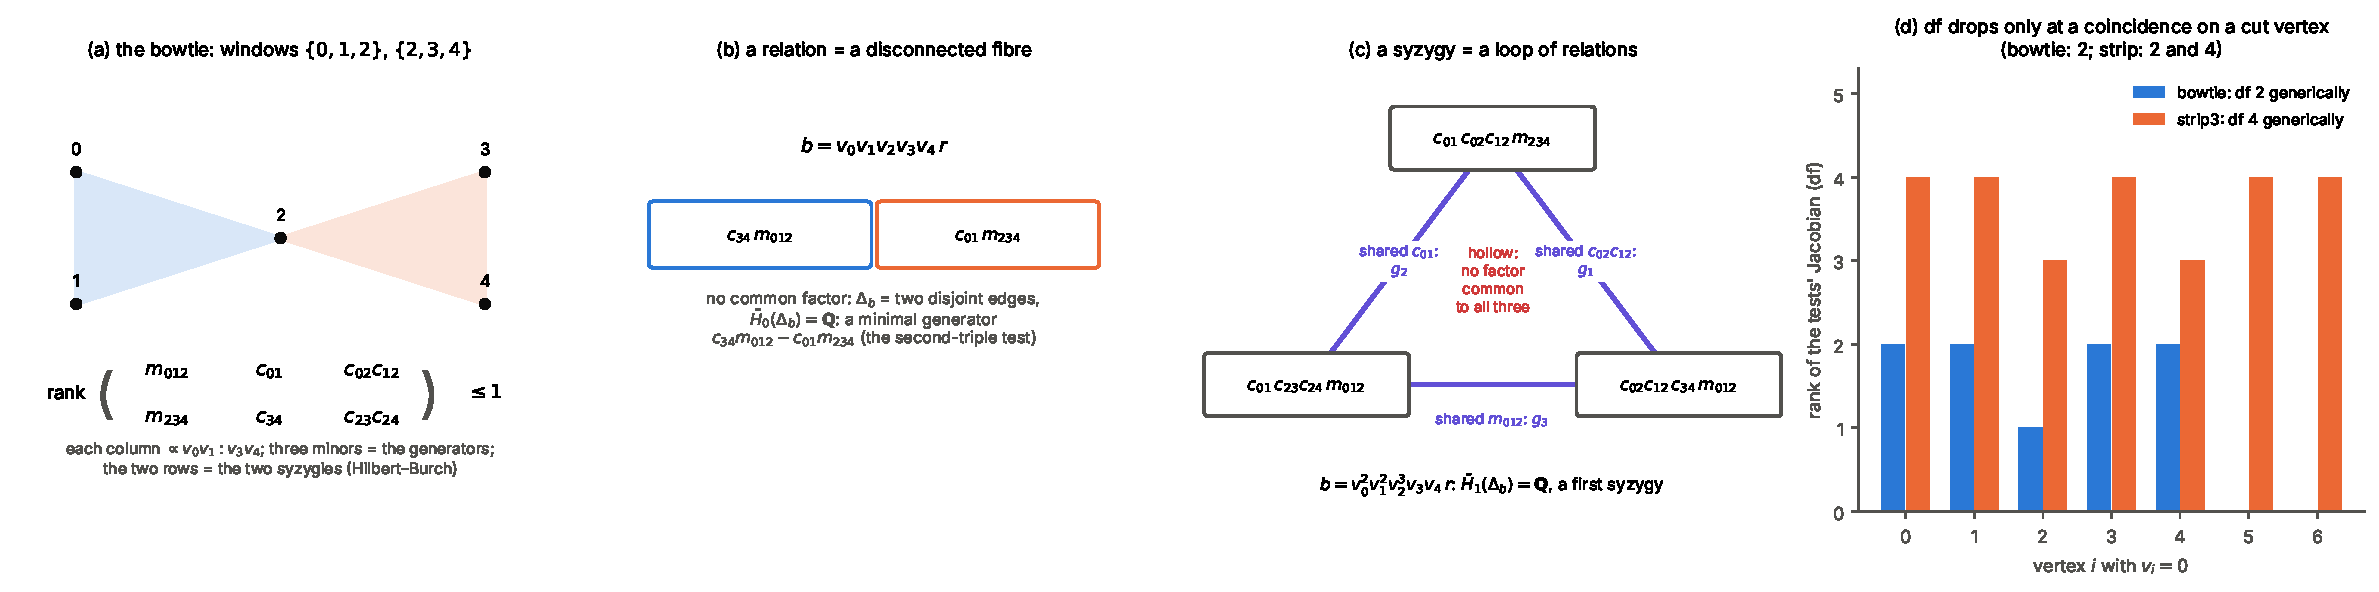
\includegraphics[width=\textwidth]{fig_syzygy.pdf}
\caption{Phase III, Stage 1, on the bowtie. (a) The cover and its Hilbert--Burch matrix. (b) The generator $g_1$: the latent monomial
$v_0v_1v_2v_3v_4r$ has two factorisations into observed moments with nothing in common. (c) A first syzygy: three factorisations of
$v_0^2v_1^2v_2^3v_3v_4r$, pairwise linked by the generators, with no common link. (d) The tests' degrees of freedom at a coincidence on
each variable: they drop only on cut variables.}\label{fig:syz}
\end{figure}

\section{Phase III, Stage 2: higher windows and the latent moment sequence}\label{sec:higher}
A window of size four or more is not monomial: $m_{0123}=v_{0123}(r^2+1)$. The polynomials $s_k(r)$ have a meaning, and once it is
seen the relations of higher windows follow.

\begin{lemma}[the standardised latent]\label{lem:latent}
Let $\tau=t$ on type 1 (probability $w$) and $\tau=-1/t$ on type 2. Then $E\tau=0$, $E\tau^2=1$, $a=\mu+v\tau$, and
\[
m_S=E\prod_{i\in S}v_i\tau=v_S\,M_{|S|},\qquad M_k=E\tau^k=s_k(r).
\]
The atoms are the roots of $\tau^2=r\tau+1$, so $M_{k+1}=rM_k+M_{k-1}$: the $s_k$ are the Fibonacci polynomials, the moments of a
two-point law.
\end{lemma}

\begin{proof}
$wt-(1-w)/t=0$ and $wt^2+(1-w)/t^2=1$ for $w=1/(1+t^2)$; $t\cdot(-1/t)=-1$ and $t-1/t=r$. Check HW1 verifies $s_k=E\tau^k$ for
$k\le8$ and $m_S=v_SM_{|S|}$ on random laws.
\end{proof}

Observing a window observes all its marginals, so a cover is a simplicial complex $K$, and the coordinates are $m_F$ for the faces with
$|F|\ge2$.

\begin{theorem}[relations of higher windows]\label{thm:higher}
\begin{enumerate}
\item[(1)] \emph{Graded pieces.} The relations form $I_K=\ker(m_F\mapsto v_FM_{|F|}(r))$, graded by the $v$-exponents. In degree $b$,
  $I_b$ is the space of linear relations among the polynomials $\prod_FM_{|F|}(r)^{u_F}$, over the monomials $u$ with $Au=b$. For pairs
  and triples these polynomials are powers of $r$, so the relations are binomials (\cref{thm:syz}). From size four on, sums appear.
\item[(2)] \emph{Fibonacci gluing.} For faces $T,T'$ with $T\cap T'=\{i,j\}$ and $T\cup T'\in K$,
\[
c_{ij}\bigl(m_{T\cup T'}-m_{T\setminus j}\,m_{T'\setminus i}\bigr)=m_T\,m_{T'} ,
\]
  from $M_{k+l-2}=M_kM_l+M_{k-1}M_{l-1}$. For two triples the left side minus the right is
  $v_Tv_{T'}\,(M_4-M_3^2-1)$, which is $v_Tv_{T'}$ times the Hankel determinant
  $\det\begin{psmallmatrix}1&0&1\\0&1&M_3\\1&M_3&M_4\end{psmallmatrix}$.
\item[(3)] \emph{Computed ideals.}
\begin{center}\small
\begin{tabular}{p{0.2\textwidth}ccp{0.25\textwidth}p{0.27\textwidth}}\toprule
cover (faces) & $n$ & codim & generators & Betti numbers (Macaulay2 $=$ Singular)\\\midrule
the full four-variable window & 11 & 6 & 16: 2 tetrads, 8 exchanges, 6 trinomials & 16, 41, 47, 40, 24, 5\\
tetrahedron $+$ triangle on an edge & 14 & 8 & 26, with cross-window trinomials & 26, 92, 171, 258, 274, 161, 44, 3\\
two tetrahedra on an edge & 21 & 14 & 71: 50 binomials, 21 trinomials & (not computed)\\
the full five-variable window & 26 & 20 & 159: 104 binomials, 45 trinomials, 10 four-term & (not computed)\\\bottomrule
\end{tabular}
\end{center}
  The four-term relations come from $M_5=r^3+2r$, for example
  $c_{01}m_{234}^2-c_{02}c_{34}m_{1234}+m_{0234}m_{1234}-m_{234}m_{01234}$.
\item[(4)] \emph{The lab's residuals.} For the full four-variable window the codimension is $6$, which is the rank of the lab's six
  residuals (two tetrads, three triple differences and the quadruple \cite[Theorem G]{Lab}). So those six are a local complete
  intersection, and the other ten generators are dependent on them through the $41$ first syzygies.
\end{enumerate}
\end{theorem}

\begin{proof}
(1) A monomial maps to $v^{Au}\prod_FM_{|F|}^{u_F}$; different $v$-degrees are independent, and within one degree the relations are
the linear relations among the $r$-polynomials. (2) The Fibonacci identity $F_{a+b}=F_{a+1}F_b+F_aF_{b-1}$ with $M_k=F_{k-1}$. Also
$v_{ij}v_{T\cup T'}=v_{ij}v_{T\setminus j}v_{T'\setminus i}=v_Tv_{T'}$. (3) Macaulay2, with every Betti table recomputed by Singular's
\texttt{sres} and \texttt{minres} \cite{Singular} (HW2, HW4). Each of the six trinomials agrees with a gluing relation modulo the tetrads,
and all of them vanish exactly in rational arithmetic on model points (HW3). (4) The Jacobian of the lab's residuals at a generic
truth has rank $6$ (HW2), and (5) of \cref{thm:syz} applies to any ideal at smooth points.
\end{proof}

\section{Three types: the proof of concept ($k=3$, $m=5$)}\label{sec:three}
\paragraph{Collinear types.} If all $k$ types lie on one line, $a_j=\mu+v\tau_j$, the pair moments have rank one, and
\cref{lem:latent} holds with a $k$-atom latent $\tau$ of mean $0$ and variance $1$. Positivity, $0\le\mu_i+v_i\tau\le1$ for every
$i$, confines $\tau$ to an interval $I=[\tau_-,\tau_+]$; the two-type walls are its ends.

\begin{proposition}[collinear $k$ types]\label{prop:collinear}
\begin{enumerate}
\item[(1)] Given the pairs, the hiding set is the set of $k$-atom laws on $I$ with $M_1=0$ and $M_2=1$. It has dimension $2k-3$: $1$ for
  two types, $3$ for three.
\item[(2)] A window of size $j$ reveals $M_j$. The sizes $3,4,\dots,2k-1$ each remove one dimension (Prony), so three types need windows
  of sizes $3$, $4$ and $5$. On $m=5$ the fibre dimension goes $3\to2\to1\to0$ (HW5).
\item[(3)] \emph{Two types are extreme.} Over all laws on $I$ with $M_1=0$ and $M_2=1$, the range of $M_3$ is exactly the two-type
  segment: the extremes are two-point laws with one atom at an end of $I$, the principal representations of the moment problem
  \cite{KarlinStudden1966,KreinNudelman1977}. So under pair-only disclosure a three-variable event has the same range for any number of
  collinear types as for two. This makes Theorem A of the lab robust to the number of types.
\item[(4)] \emph{Two types are a boundary.} $M_4\ge M_3^2+1$, with equality iff $\tau$ has two atoms. Two types are the lower boundary of
  the $(M_3,M_4)$ moment space, and the gluing trinomial of \cref{thm:higher}(2) is its equation. Since the trinomial equals
  $v_Tv_{T'}(M_4-M_3^2-1)$ and the sign of $v_Tv_{T'}$ is known from the pairs, the lab's quadruple residual becomes a \emph{one-sided} test
  for more than two collinear types.
\end{enumerate}
\end{proposition}

\begin{proof}
(1) $k$ atoms and $k$ weights, less one normalisation and two moment conditions. (2) Moments up to $2k-1$ determine a generic $k$-atom law.
(3) For a linear functional of $M_3$ under the three equality constraints, a basic optimal solution of the moment linear programme has at most
three atoms; the principal representations of $(M_0,M_1,M_2)$ on an interval are two-point laws. Check HW6 solves the programme on a grid of
$6001$ support points: the range of $M_3$ is $[-0.7626,\,0.5731]$, equal to the two-type segment to $10^{-5}$. (4) The Hankel matrix
of a law is positive semidefinite, and it is singular iff the law has at most two atoms. Given $M_3=-0.408$, $M_4$ is pinned at
$1.1667$ for two types and ranges over $[1.1667,\,1.8900]$ for three or more (HW6).
\end{proof}

\paragraph{General three types.} Without collinearity, $c=VV^\top$ off the diagonal with $V\in\R^{5\times2}$ (the types span a
plane), and the freedom of $V$ is $O(2)$. This is the continuous analogue of the two-type sign group $O(1)=\{\pm1\}$.

\begin{proposition}[three types on five variables; computed]\label{prop:three}
\begin{enumerate}
\item[(1)] \emph{Pairs.} The only relation among the ten pair moments is the pentad, a single generator of degree $5$ with $12$ terms
  \cite{DrtonSturmfelsSullivant2007}. It vanishes on three-type pair moments and not on random ones. The image has rank $14$ of $17$, so the
  hiding set has dimension $3$.
\item[(2)] \emph{The window ladder.} Adding triples gives ranks $15,16,16,17$; four suitable triples, or all ten, already identify a
  generic three-type law locally. The third triple, $\{0,1,4\}$, adds nothing: rank depends on how the windows overlap, not only on how many
  there are. For two types, pairs and one triple suffice.
\item[(3)] \emph{$S_3$ descent creates identifiability.} A single four-variable window is defective: rank $13$ of $14$, a curve of
  explanations. This is the known dimension deficiency of the three-class model on four binary variables \cite{GeigerHeckermanKingMeek2001}.
  Two windows $\{0,1,2,3\}$ and $\{1,2,3,4\}$ overlapping in a triple have rank $17$. Multistart fitting of the glued data finds one
  solution up to label permutation ($32$ converged starts). The two local curves meet only where the labels match on the overlap, and the
  transition $\pi\in S_3$ is the unique permutation matching $(w_j,a_j|_{\{1,2,3\}})$. Gluing the windows identifies what neither identifies
  alone.
\item[(4)] \emph{The non-abelian coincidence.} If two types have equal weight and agree on the overlap, the overlap data have stabiliser
  $S_2$ and the rank falls to $14$: the transition is ambiguous and a continuum of glued laws appears. This is the three-type analogue of
  \cref{ex:zero}, where a coincidence created a scale.
\end{enumerate}
\end{proposition}

\paragraph{Decisions.} \Cref{fig:higher}(c) compares what a decision can rely on when the truth is the two-type law of the lab's worked example,
for $E_3$ (all of $0,1,2$ harmed; truth $0.0130$) and $E_4$ (all of $0,\dots,3$; truth $0.0086$).
\begin{itemize}
\item Under pairs only, $E_3$ ranges over $[0.0068,0.0153]$ for two types, the same interval for collinear three types (by
  \cref{prop:collinear}(3)), and at least $[0.0013,0.0160]$ for general three types. Non-collinear explanations give each variable its
  own second latent direction.
\item With the triple $\{0,1,2\}$, $E_3$ is read off directly. $E_4$ is then pinned at $0.0086$ for two types. For collinear three types
  it lies in $[0.0075,0.0086]$, exactly by linear programming; for general three types it lies in at least $[0.0068,0.0100]$, an inner
  bound from constrained optimisation.
\end{itemize}
So the number of types decides the probe sizes a settled decision needs. For two types, triples settle every event. For three, an event
on four variables needs a four-window. Model size is a decision-relevant assumption, and the one-sided test of
\cref{prop:collinear}(4) is how the data can speak to it.

\begin{figure}[t]\centering
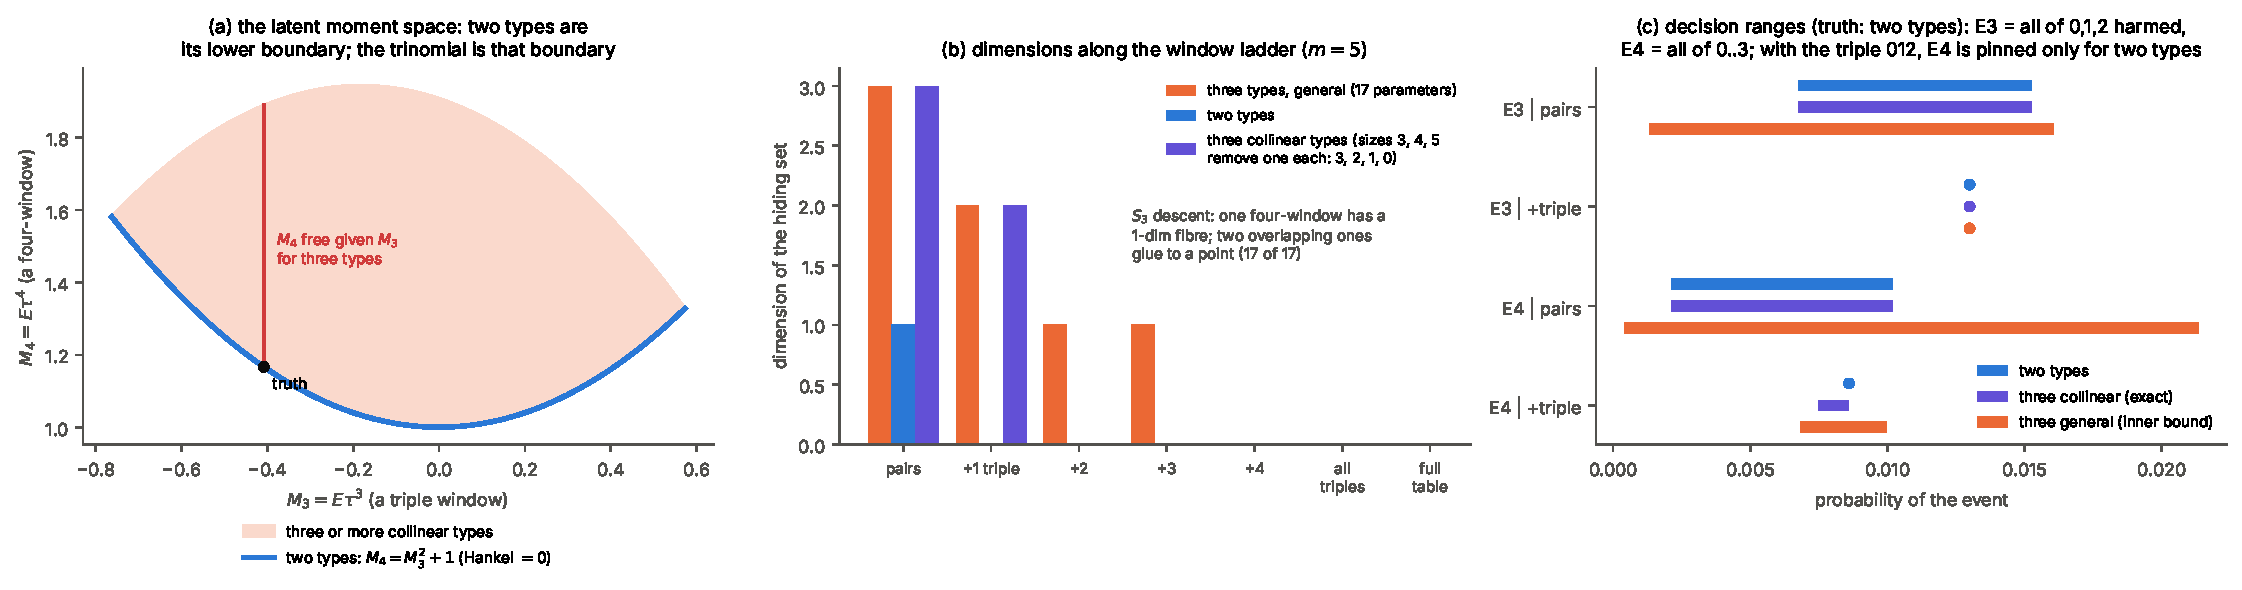
\includegraphics[width=\textwidth]{fig_higher.pdf}
\caption{Higher windows and three types. (a) The moment space of the standardised latent on the positivity interval. Two types are the
lower boundary $M_4=M_3^2+1$, where the gluing trinomial vanishes; three or more collinear types fill the region above. (b) Hiding
dimensions along the window ladder for a generic three-type truth on $m=5$, for two types, and for collinear three types. (c) Decision
ranges at a two-type truth under two-type, collinear three-type (exact) and general three-type (inner bound) explanations.}\label{fig:higher}
\end{figure}

\section{Phase III, Stage 3: real signs, sheets and the syzygies of sign tests}\label{sec:signs}
Over the reals the explanations come in sheets, and the data carry signs. This section says how the two are linked, and how the
syzygies of Stage 1 govern the sign tests.

\paragraph{The parity matrix.} Since $s_k(-r)=(-1)^ks_k(r)$, a sign change $\sigma\in\{\pm1\}^{m+1}$ of $(v_0,\dots,v_{m-1},r)$ preserves
every observed moment iff $\prod_{i\in F}\sigma_i\,\sigma_r^{|F|}=1$ for every face $F$. Over $\mathbb F_2$ this reads $P^\top\sigma=0$. The
\emph{parity matrix} $P$ has one column $1_F+(|F|\bmod2)\,e_r$ per face; for pairs and triples it is the extended incidence matrix
$A$ reduced mod $2$.

\begin{theorem}[signs]\label{thm:signs}
\begin{enumerate}
\item[(1)] \emph{Sheets.} The sign symmetries form $G_2=\ker P^\top$, computed on the coordinates that occur in some face (a coordinate
  that occurs nowhere is continuous). The label swap, all signs flipped, always lies in $G_2$. Over generic data the real fibre is $|G_2|$
  translates of one connected piece, and the sheets before positivity are $G_2/\langle\text{swap}\rangle$. For pair-only covers this is
  the $2^{c^*-1}$ of \cref{thm:hiding}(4).
\item[(2)] \emph{Relative signs.} A product of signs $\prod_{i\in S}\sigma_i$ is fixed by the cover iff it is constant on $G_2$, which is
  a linear condition over $\mathbb F_2$. A window meeting two components in odd numbers fixes their relative sign, and one meeting them
  in even numbers does not. Windows that each meet only one component can also fix it, through the shared $r$ (\cref{ex:signs}). The
  odd-meeting rule stated in the earlier draft is therefore only a special case.
\item[(3)] \emph{Visible and invisible sign classes.} For pairs and triples, the data sign patterns that pass every relation's sign test
  form $(L\bmod2)^\perp$, with $2^{\,n-\operatorname{codim}}$ elements. The patterns realised by real explanations form
  $\operatorname{im}P^\top$, with $2^{\operatorname{rank}_2A}$ elements. The quotient, the \emph{invisible} classes, has
  $2^{\operatorname{rank}_\mathbb QA-\operatorname{rank}_2A}$ elements. Its exponent is the number of even invariant factors of the Smith
  form of $A$, the $2$-torsion of $\operatorname{coker}A$. For a pair graph,
\[
b_1(G)=\underbrace{\operatorname{codim}I_B}_{\text{visible: sign shadows of relations}}+\underbrace{\#\{\text{non-bipartite components}\}}_{\text{invisible: the odd-cycle classes}} ,
\]
  so the lab's sign group $H^1(\Gamma;\mathbb Z/2)$ \cite[Theorem M]{Lab} splits into classes the relations see and classes no relation
  can see.
\item[(4)] \emph{Syzygies govern the sign tests.} A binomial generator $g_j=x^{u_j}-x^{w_j}$ imposes the sign test
  $\langle u_j-w_j,s\rangle\equiv0$. Evaluated at the identity of the torus (all moments $1$, which is a model point), the first syzygies
  are integer relations $\sum_jh_j(1)(u_j-w_j)=0$, of rank $\#\text{gens}-\operatorname{codim}$ over $\mathbb Q$ and over $\mathbb F_2$.
  So exactly $\operatorname{codim}$ sign tests are independent, and the syzygies say which are redundant.
\item[(5)] \emph{Sheets and relations trade.} Adding a face changes $\dim G_2$ by $-\Delta\operatorname{rank}_2P$ and the number of
  invisible classes by $\Delta\operatorname{rank}_\mathbb QA-\Delta\operatorname{rank}_2A$. The four possible steps are:
  \begin{itemize}
  \item $(1,1)$: a freedom is absorbed and a sign fixed;
  \item $(0,0)$: a new test that carries no sign information;
  \item $(1,0)$: a freedom is absorbed but an invisible class is born, which happens exactly when an edge closes an odd cycle;
  \item $(0,1)$: a new test whose sign shadow kills a pair of sheets and turns an invisible class into a visible one.
  \end{itemize}
  A sheet the latent side loses is a sign test the data side gains.
\end{enumerate}
\end{theorem}

\begin{proof}
(1) $\sigma$ acts by multiplication and preserves each $m_F$ iff the parity condition holds. Over generic data with all moments non-zero,
the fibre of the parametrisation is a torsor under $\{z:z^{a_j}=1\}=K_+\times G_2$, with $K_+$ the connected positive part. All ones
is in $G_2$ because $|F|+|F|$ is even. (2) $\prod_{i\in S}\sigma_i$ is invariant iff it is trivial on $G_2$. (3) The sign of a
monomial $x^u$ at the sign pattern $s$ is $\langle u,s\rangle$. The model's patterns are the image of $\sigma\mapsto P^\top\sigma$.
Generators of $I_A$ form a Markov basis, which spans the saturated lattice $L=\ker_\mathbb ZA$, so the patterns passing every test form
$(L\bmod2)^\perp$, of dimension $n-\operatorname{codim}=\operatorname{rank}_\mathbb QA$. Over $\mathbb F_2$ the rank of $A$ counts its odd
invariant factors. For a graph, $\operatorname{rank}_\mathbb QB=m-b$ and $\operatorname{rank}_2B=m-c$, with $b$ the bipartite and $c$
all components; $b_1=|E|-m+c$ and $\operatorname{codim}I_B=|E|-m+b$. (4) As in \cref{thm:syz}(5), differentiate $\sum_jh_jg_j=0$ at the
smooth point $1$, where $\nabla g_j(1)=u_j-w_j$ (up to the sign of $g_j$). The kernel of $\mathbb Z^{\#\text{gens}}\to L$ is saturated, so its
reduction mod $2$ has the same rank. (5) Rank bookkeeping. An edge raises $\operatorname{rank}_\mathbb QB$ but not $\operatorname{rank}_2B$
iff it joins two vertices on the same side of a bipartite component.
\end{proof}

Checks SG1--SG8 verify the theorem.
\begin{itemize}
\item On six covers with finite fibres, multistart real solving finds exactly $|G_2|$ solutions.
\item On the zoo, $b_1$ splits as stated.
\item On the Stage 1 covers, enumerating all data sign patterns gives the counts of (3): $256$ pass and $128$ are realised on the strip;
  $8$ and $4$ on the triangle.
\item The syzygies evaluated at the identity have the ranks of (4).
\item On $300$ random covers, $1136$ added faces fall into the four steps of (5) ($522$, $592$, $22$, $2$). Every $(1,0)$ step is an edge
  closing an odd cycle.
\end{itemize}

\begin{example}[two triangles that share only $r$: a reader's guide]\label{ex:signs}
Take triangles $A=\{0,1,2\}$ and $B=\{3,4,5\}$, all six pairs, and the triple $\{0,1,2\}$.
\begin{enumerate}
\item \emph{Parity.} The pair columns force $\sigma_0=\sigma_1=\sigma_2$ and $\sigma_3=\sigma_4=\sigma_5$. The triple $\{0,1,2\}$ gives
  $\sigma_0\sigma_1\sigma_2\sigma_r=1$, so $\sigma_r=\sigma_A$. Then $G_2$ has basis $(1,1,1,0,0,0,1)$ and $(0,0,0,1,1,1,0)$, four elements and
  two sheets: triangle $B$'s labels can be swapped on their own. Real solving finds $4$ solutions (SG1).
\item \emph{Add the triple $\{3,4,5\}$.} Now $\sigma_r=\sigma_B$ as well, so $\sigma_A=\sigma_B$. $G_2$ is just the swap, there is one sheet,
  and $2$ solutions. No window meets both triangles; the alignment travels through the weight they share.
\item \emph{The relation it brings.} The new relation is $c_{34}c_{35}c_{45}\,m_{012}^2=c_{01}c_{02}c_{12}\,m_{345}^2$: both triples must
  report the same $r$. Its sign test is $\operatorname{sgn}(c_{34}c_{35}c_{45})=\operatorname{sgn}(c_{01}c_{02}c_{12})$. Before, the two
  triangles' odd-cycle classes were both invisible ($2^2$ invisible patterns). Now their difference is visible, and only their common
  class is not ($2^1$). This is the $(0,1)$ step: one sheet pair lost on the latent side, one sign test gained on the data side.
\item \emph{The liar, for contrast.} On a single triangle the patterns with $c_{01}c_{12}c_{02}<0$ satisfy every relation (there are
  none) yet have no real explanation (\cref{fig:signs}(b)). The Smith form $(1,1,2)$ of the incidence matrix records this class: an
  obstruction that lives only in the signs, never in the ideal.
\end{enumerate}
\end{example}

\begin{figure}[t]\centering
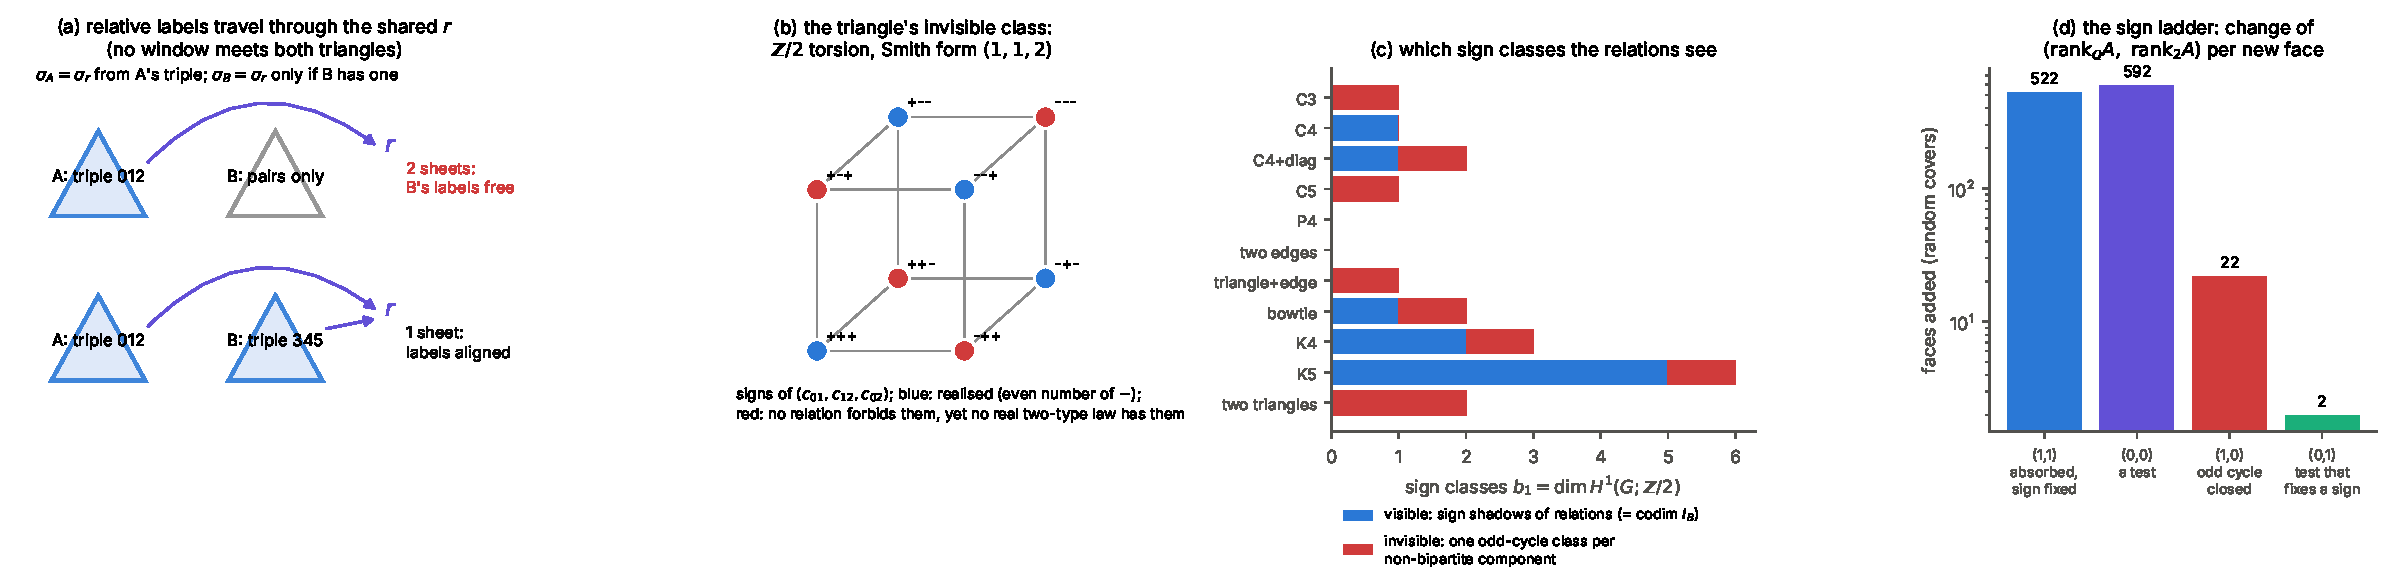
\includegraphics[width=\textwidth]{fig_signs.pdf}
\caption{Real signs (\cref{thm:signs}, \cref{ex:signs}). (a) Two disjoint triangles: one triple leaves the second triangle's labels free,
and a triple on each aligns them through the shared $r$. (b) The triangle's eight data sign patterns: four realised, four allowed by every
relation but realised by nothing. (c) Over the zoo, $b_1$ splits into visible classes (sign shadows of relations) and invisible ones (one
odd-cycle class per non-bipartite component). (d) The sign ladder over random covers: what one new face does to
$(\operatorname{rank}_\mathbb QA,\operatorname{rank}_2A)$.}\label{fig:signs}
\end{figure}

\begin{remark}[sheets, the tangent structure and pooling]
The tangent companion \cite{Tangent} uses these sheets. Each sheet is an object of its cone category, the layers are the walls, and a
worst-case decision over a sheet is certified by the tangent cone at its minimiser. Pooling two data sets can leave the two-type domain:
the pooled pair covariances can take a negative product around a triangle, which is the invisible odd-cycle class of \cref{thm:signs}(3).
That is the main way pooling fails globally \cite[Theorem ``pooling along a chord'']{Tangent}.
\end{remark}

\section{Phase III, Stage 4: strata}\label{sec:strata}
In the model a zero pair moment is a coincidence ($c_{ij}=v_iv_j=0$ forces $v_i=0$ or $v_j=0$). So the strata are:
\begin{itemize}
\item sets $Z$ of coincident variables ($v_i=0$ for $i\in Z$);
\item equal weights ($r=0$);
\item the merge ($v=0$).
\end{itemize}
These are the layers of the tangent companion: each stratum is a smaller cover in its own right, and the deepest one, the merge, needs a
blow-up.

\begin{theorem}[strata]\label{thm:strata}
\begin{enumerate}
\item[(1)] \emph{Latent rank.} At a point with zero set $Z$ and $r\ne0$, the Jacobian of $(v,r)\mapsto(m_F)$ has rank
\[
\operatorname{rank}A_{K\setminus Z}+\#\{j\in Z:\ \text{some face }F\text{ has }F\cap Z=\{j\}\} ,
\]
  where $A_{K\setminus Z}$ is the extended incidence matrix of the faces avoiding $Z$. Faces meeting $Z$ twice vanish to second order;
  faces meeting it once contribute the direction $e_j$. The hiding dimension there is $m+1$ minus this rank.
\item[(2)] \emph{Tests.} A generator whose $A$-degree in $i$ (the number of its factors containing $i$) is at least $2$ vanishes to
  second order at $v_i=0$. The tests' degrees of freedom there are the rank of the generators of degree at most $1$ in $i$.
\item[(3)] \emph{Pair graphs.} At $v_i=0$ the tests lose $\max(0,\ \ell_i-1)$ degrees of freedom, where the \emph{lobes} $\ell_i$ count
  the components of $G-i$ that are non-bipartite together with $i$. We prove that at least this many are lost; equality holds in every
  case tested.
\item[(4)] \emph{The cut-variable conjecture, refined.} Being a cut vertex is not enough: two $4$-cycles sharing a vertex lose nothing.
  What is lost is one degree of freedom per extra non-bipartite lobe: $1$ on the bowtie, $2$ on a windmill of three triangles.
\item[(5)] \emph{Equal weights.} At $r=0$ every odd window has $m_T=0$ and carries no sign, so the sheet group is that of the even faces.
  Labels that were aligned through $r$ come apart.
\item[(6)] \emph{The merge.} At $v=0$ the latent rank and every test gradient are $0$, for every cover.
\end{enumerate}
\end{theorem}

\begin{proof}
(1) $\partial m_F/\partial v_j=m_F/v_j$ away from $Z$. At the stratum, a face with $|F\cap Z|\ge2$ has all first derivatives zero, and a face
with $F\cap Z=\{j\}$ has only $\partial_{v_j}m_F=v_{F\setminus j}\,s_{|F|}(r)\ne0$. The remaining rows are the usual logarithmic rows of the
faces avoiding $Z$, with $r$ entering every higher window since $s_k'(r)\ne0$ generically. (2) A monomial with two vanishing factors has
zero gradient. A binomial is homogeneous in the $A$-grading, so both of its monomials have the same degree in $i$. (3) Two odd cycles in
different lobes are joined only through $i$, so each figure-eight relation between lobes visits $i$ twice ($A$-degree $2$). There are
$\ell_i-1$ independent ones, all vanishing to second order by (2). That fewer are lost is not proved in general; checks CS4 confirm equality
on $109$ random graphs and four named ones. (5) At $r=0$, $m_T=v_Ts_{|T|}(0)=0$ for odd $|T|$, so those faces impose no sign condition.
(6) Every face meets $Z=V$ at least twice.
\end{proof}

Checks CS1--CS8 verify the theorem.
\begin{itemize}
\item The latent-rank rule holds in $294$ single and $594$ double coincidences on random covers.
\item The degree rule holds on every generator of the random covers tested.
\item Real solving confirms the equal-weight split: two disjoint triangles with their triples have $2$ explanations for $r\ne0$ and $4$ at
  $r=0$, while $K_4$ with its triples keeps $2$.
\end{itemize}

\begin{example}[the bowtie, stratum by stratum]\label{ex:strata}
For the bowtie with both triples (\cref{fig:strata}(a)), a coincidence on $0,1,3$ or $4$ costs nothing: the latent rank stays $6$ and the
tests keep $2$ degrees of freedom. A coincidence on the shared variable $2$ drops the latent rank to $3$, so the hiding set becomes
three-dimensional. It also drops the tests to $1$: the closed walk through $2$ and one form of the second-triple test vanish to second
order, and only $c_{34}m_{012}=c_{01}m_{234}$ survives. At $r=0$ nothing is lost here, because the two triangles share variable $2$
and are aligned by the pairs. Two disjoint triangles aligned only through $r$ would split (\cref{fig:strata}(c)). At the merge
everything is lost. This is the lab's worthless probe and its $n^{-1/4}$ tempo, located exactly.
\end{example}

\begin{figure}[t]\centering
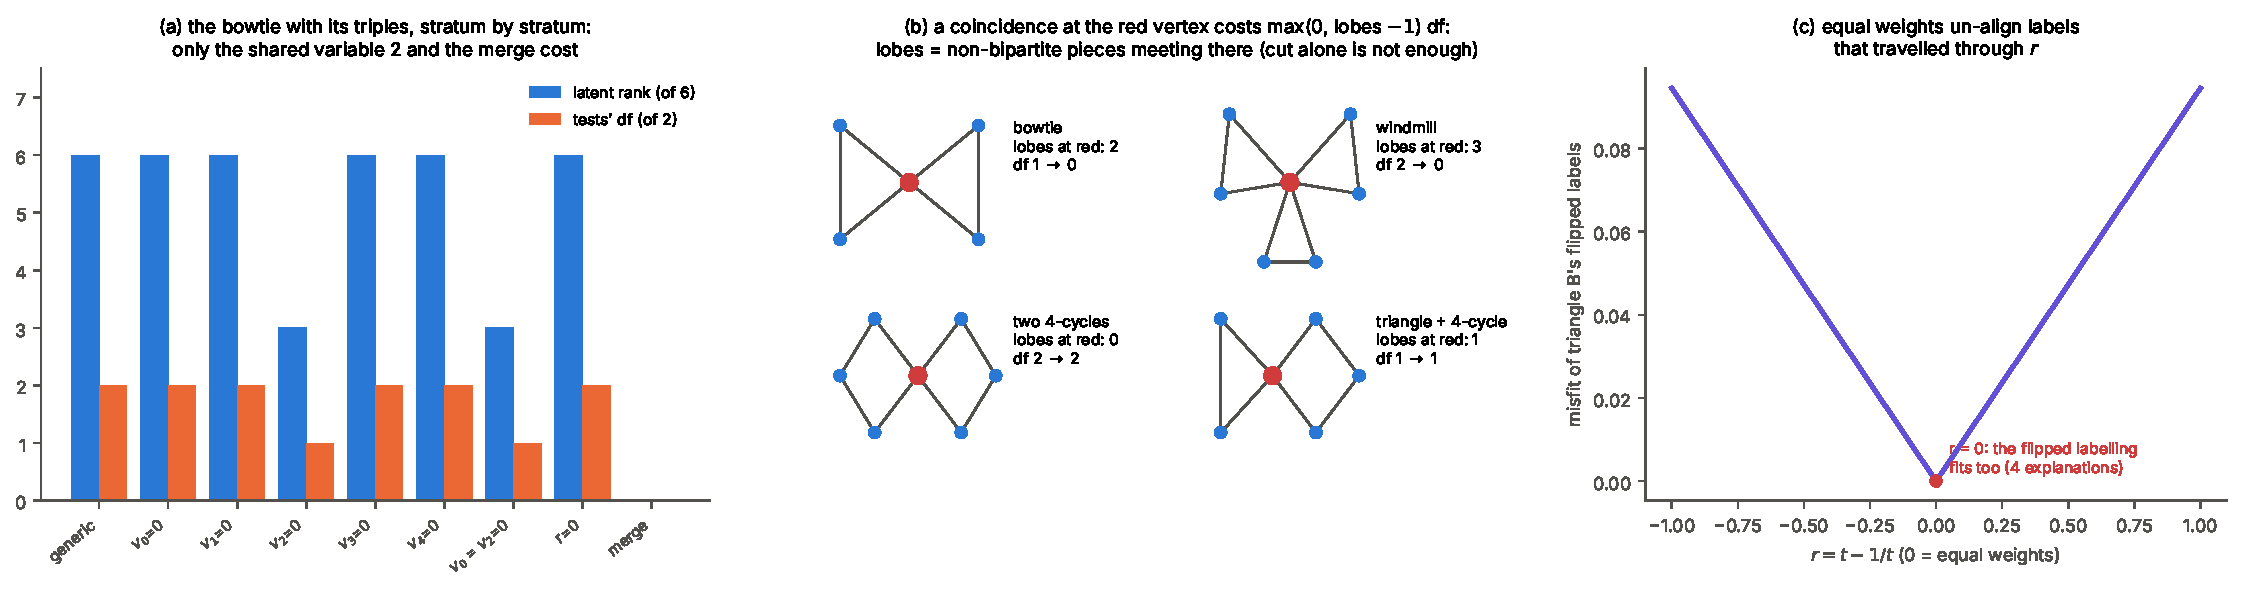
\includegraphics[width=\textwidth]{fig_strata.pdf}
\caption{Strata (\cref{thm:strata}). (a) The bowtie with its triples: latent rank and the tests' degrees of freedom on every stratum.
(b) A coincidence at the red vertex costs $\max(0,\text{lobes}-1)$ degrees of freedom. A cut vertex between bipartite pieces costs nothing.
(c) The misfit of the explanation with triangle $B$'s labels flipped, for two disjoint triangles with their triples. It vanishes only at
$r=0$.}\label{fig:strata}
\end{figure}

\section{Where the two-type theory on covers now stands}\label{sec:shape}
Phase III is complete. The table records, for any cover (a simplicial complex of observed windows), what each layer of structure is, how
it is computed, and where it changes.

\begin{center}\small
\begin{tabular}{p{0.15\textwidth}p{0.36\textwidth}p{0.38\textwidth}}\toprule
layer & what it is & how it is computed / where it changes\\\midrule
existence & factorisation of the pairs; sign class; modulus class; positivity & \cref{thm:factor}: zero strata, $H^1(G;\mathbb Z/2)$, $\operatorname{coker}B$, the walls\\
continuous freedom & weight $t$, one scale per bipartite component, free variables & $m+1-\operatorname{rank}_\mathbb QA$; hiding polytopes with facets of slope $\pm1$ (\cref{thm:hiding})\\
relations & tests among the observed moments & toric ideal for pairs and triples (\cref{thm:syz}); Fibonacci--Hankel relations for higher windows (\cref{thm:higher})\\
syzygies & dependencies among the tests & the tests have $\operatorname{codim}$ degrees of freedom; homology of $\Delta_b$; at the torus identity, dependencies among sign tests (\cref{thm:signs}(4))\\
sheets & discrete label freedom & $G_2=\ker P^\top$ over $\mathbb F_2$; relative signs by linear algebra; visible versus invisible classes ($2$-torsion of $\operatorname{coker}A$)\\
strata & where ranks drop & latent rank by faces avoiding $Z$; tests by $A$-degree; lobes on pair graphs; $r=0$ un-aligns; the merge (\cref{thm:strata})\\
more types & collinear $k$ types; three types on five variables & moment spaces, window sizes $3,\dots,2k-1$; pentad, $O(2)$, $S_3$ descent (\cref{prop:collinear,prop:three})\\\bottomrule
\end{tabular}
\end{center}

What remains is consolidation, not new structure:
\begin{itemize}
\item \emph{Phases IV--V.} The three notions of identifiability (factorisation, parameters, law) and the walls, read off this table.
\item The Betti tables of the two largest covers.
\item The general three-type theory on arbitrary covers.
\end{itemize}

\section{What comes next}\label{sec:next}
\paragraph{Loose ends of Phase III.} Prove equality in \cref{thm:strata}(3); a lobe rule for covers with windows (where $r$ joins
lobes, as in \cref{ex:signs}); the Betti tables of the two largest covers.

\paragraph{Phases IV--V.} Separate factorisation, parameter and distribution identifiability; list the walls where sheets lose
dimension.

\paragraph{Three types on arbitrary covers.} Replace the sign cocycle by an $O(2)$-valued one on the pair layer, and the label sheets by
$S_3$-torsors on the window nerve. The cocycle condition around a cycle of three windows is the first place where a genuinely
non-abelian obstruction can appear.

\section*{Checks}
Phases I--II are checked in \texttt{engine/check\_covers.py} (module \texttt{engine/pce/covers.py}; $9/9$, under two minutes).
Phase III, Stage 1 is checked in \texttt{engine/check\_syzygy.py} (module \texttt{engine/pce/syzygy.py}; $8/8$, about thirty seconds;
needs Macaulay2). Stage 2 and the three-type proof of concept are checked in \texttt{engine/check\_higher.py} (modules
\texttt{engine/pce/syzygy.py}, \texttt{engine/pce/threetype.py}; $8/8$, a few minutes; needs Macaulay2 and Singular). The decision
ranges of \cref{fig:higher}(c) for general three types come from \texttt{covers/fig\_higher.py} and a constrained-optimisation run
recorded with it; they are inner bounds. Stage 3 is checked in \texttt{engine/check\_signs.py} (module \texttt{engine/pce/signs.py};
$8/8$; needs Macaulay2), and Stage 4 in \texttt{engine/check\_cover\_strata.py} (module \texttt{engine/pce/cover\_strata.py}; $8/8$). \Cref{lem:bridge} is checked in
\texttt{engine/check\_bridge.py} ($5/5$; needs Macaulay2).
\begin{center}\small
\begin{tabular}{lp{0.8\textwidth}}\toprule
CV1 & rank $B_G=|V|-b(G)$ on $300$ random graphs\\
CV2 & existence criterion against a direct non-linear solve: $66/66$ (44 factorisable, 15 sign-class and 7 modulus-class failures)\\
CV3 & factorisation set and its tangent dimension on the zoo\\
CV4 & zero strata: coincidence on the triangle creates a scale; zero edge inside $N$ infeasible\\
CV5 & every sampled point of every sheet rebuilds the observed singles and pairs; each facet is a named wall\\
CV6 & connected bipartite graphs: rectangles in $(\log\lambda t,\log\lambda/t)$\\
CV7 & dimension $b(G)+1$ on all eleven zoo graphs; sheet counts\\
CV8 & $K_3$ recovers the lab's segment exactly\\
CV9 & a sheet emptied by positivity\\\midrule
SZ1 & generators vanish on the model and not off it; $\operatorname{codim}=n-\operatorname{rank}A$\\
SZ2, SZ3 & all multigraded Betti numbers equal Hochster's formula; none missed up to $|u|\le4$\\
SZ4 & pair part $=I_B$, the even closed walks, codimension $|E|-\operatorname{rank}B$\\
SZ5 & the test ladder: each triple adds $0$ or $1$\\
SZ6 & bowtie: Hilbert--Burch, syzygies the rows of $N$\\
SZ7 & syzygies span the left kernel of the tests' Jacobian; degrees of freedom drop at cut-variable coincidences\\
SZ8 & Cohen--Macaulay; Betti tables\\\midrule
HW1 & $s_k=E\tau^k$; $\tau^2=r\tau+1$; $m_S=v_SM_{|S|}$\\
HW2 & the full four-window: 2 tetrads, 8 exchanges, 6 trinomials; Betti (M2 $=$ Singular); lab residuals rank $6$\\
HW3 & gluing relations exact; trinomials $=$ gluing relations modulo tetrads; Hankel\\
HW4 & tetrahedron $+$ triangle: cross-window trinomials; Betti (M2 $=$ Singular)\\
HW5 & collinear three types: fibre $3\to2\to1\to0$ with window sizes $3,4,5$\\
HW6 & moment space: $M_3$ range $=$ two-type segment; $M_4$ given $M_3$ an interval for three types\\
HW7 & pentad; the three-type ladder $14,15,16,16,17$\\
HW8 & one four-window defective; two overlapping ones identify ($S_3$ descent); coincidence rank $14$\\\midrule
SG1, SG2 & sheets $=|G_2|$ real solutions; relative labels through $r$\\
SG3 & the $\mathbb F_2$ criterion versus the odd-meeting rule\\
SG4, SG5 & invisible classes $=$ even Smith invariants; $b_1=$ visible $+$ invisible\\
SG6 & data sign patterns: passing $2^{n-\operatorname{codim}}$, realised $2^{\operatorname{rank}_2A}$\\
SG7 & syzygies at the torus identity: the dependencies among sign tests\\
SG8 & the sign ladder\\\midrule
BR1--BR5 & \cref{lem:bridge}: image ideal, torus fibre, real translates, positive part $=$ sheet; the nesting; walls on a sheet\\\midrule
CS1, CS2 & latent rank at single and double coincidences\\
CS3 & tests: degree $\ge2$ generators vanish to second order\\
CS4, CS5 & pair graphs: $\max(0,\text{lobes}-1)$; the cut-variable conjecture refined\\
CS6 & equal weights un-align labels aligned through $r$\\
CS7 & the merge: rank $0$, df $0$\\
CS8 & the bowtie's strata table\\\bottomrule
\end{tabular}
\end{center}

\begin{thebibliography}{9}
\bibitem{Lab} V.~K.~Awasthi, A lab for latent actors: hiding segments, probes, settled decisions, injected records and sources, 2026.
\bibitem{DrtonSturmfelsSullivant2007} M.~Drton, B.~Sturmfels and S.~Sullivant, Algebraic factor analysis: tetrads, pentads and beyond, \emph{Probab. Theory Related Fields} \textbf{138} (2007) 463--493.
\bibitem{Eisenbud1995} D.~Eisenbud, \emph{Commutative Algebra with a View Toward Algebraic Geometry}, Springer, 1995.
\bibitem{M2} D.~R.~Grayson and M.~E.~Stillman, Macaulay2, a software system for research in algebraic geometry, \url{https://macaulay2.com}.
\bibitem{Hochster1972} M.~Hochster, Rings of invariants of tori, Cohen--Macaulay rings generated by monomials, and polytopes, \emph{Ann. of Math.} \textbf{96} (1972) 318--337.
\bibitem{MillerSturmfels2005} E.~Miller and B.~Sturmfels, \emph{Combinatorial Commutative Algebra}, Springer, 2005.
\bibitem{OhsugiHibi1999} H.~Ohsugi and T.~Hibi, Toric ideals generated by quadratic binomials, \emph{J. Algebra} \textbf{218} (1999) 509--527.
\bibitem{Sturmfels1996} B.~Sturmfels, \emph{Gröbner Bases and Convex Polytopes}, American Mathematical Society, 1996.
\bibitem{Villarreal1995} R.~H.~Villarreal, Rees algebras of edge ideals, \emph{Comm. Algebra} \textbf{23} (1995) 3513--3524.
\bibitem{GeigerHeckermanKingMeek2001} D.~Geiger, D.~Heckerman, H.~King and C.~Meek, Stratified exponential families: graphical models and model selection, \emph{Ann. Statist.} \textbf{29} (2001) 505--529.
\bibitem{KarlinStudden1966} S.~Karlin and W.~J.~Studden, \emph{Tchebycheff Systems: With Applications in Analysis and Statistics}, Interscience, 1966.
\bibitem{KreinNudelman1977} M.~G.~Krein and A.~A.~Nudel'man, \emph{The Markov Moment Problem and Extremal Problems}, American Mathematical Society, 1977.
\bibitem{Singular} W.~Decker, G.-M.~Greuel, G.~Pfister and H.~Schönemann, \textsc{Singular}, a computer algebra system for polynomial computations, \url{https://www.singular.uni-kl.de}.
\bibitem{Tangent} V.~K.~Awasthi, A tangent structure for injected data: feasible cones, universality at corners, jets on the tetrad scheme, and decision boundaries, companion paper, 2026.
\end{thebibliography}
\end{document}
